\documentclass[11pt]{article}

\usepackage[letterpaper,margin=0.78in]{geometry}
\usepackage{microtype}
\usepackage{booktabs}
\usepackage{tabularx}
\usepackage{array}
\usepackage{amsmath}
\usepackage{xcolor}
\usepackage{tikz}
\usetikzlibrary{arrows.meta,positioning,fit,backgrounds,calc}
\usepackage{enumitem}
\usepackage{hyperref}

\definecolor{InstanceBlue}{HTML}{DCECF8}
\definecolor{InstanceLine}{HTML}{3D759E}
\definecolor{HarnessGreen}{HTML}{E4F1E7}
\definecolor{HarnessLine}{HTML}{4E7C5B}
\definecolor{EvidenceGreen}{HTML}{F1F7F2}
\definecolor{Ink}{HTML}{24313A}
\definecolor{LinkBlue}{HTML}{245E88}
\definecolor{AlertRed}{HTML}{9E3F3F}

\hypersetup{
  colorlinks=true,
  linkcolor=LinkBlue,
  urlcolor=LinkBlue,
  citecolor=LinkBlue,
  pdftitle={A Claim-Coupled Verification Method for Hard Identification Problems},
  pdfauthor={}
}

\setlength{\parindent}{1em}
\setlength{\parskip}{0.2em}
\setlength{\emergencystretch}{2em}
\renewcommand{\arraystretch}{1.12}
\raggedbottom

\newcolumntype{Y}{>{\raggedright\arraybackslash}X}
\newcommand{\code}[1]{\texttt{#1}}
\newcommand{\exchangeable}{\textbf{\textcolor{InstanceLine}{EXCHANGEABLE}}}
\newcommand{\fixedarena}{\textbf{\textcolor{HarnessLine}{FIXED}}}

\title{A Claim-Coupled Verification Method for Hard Identification Problems}
\author{}
\date{Version 0.2 --- 2026-07-24}

\begin{document}
\maketitle

\begin{abstract}
This report describes a two-layer method for hard
identification-and-construction problems.  Layer A is an autonomous research
arena: independent contestant agents pursue discovery under adversarial peer
verification, while a sovereign daemon mediates an append-only blackboard and
a sealed oracle.  Layer B is a claim-coupled evidence kit: independent
constructions, deterministic gates, provenance checks, laddered claim
statuses, and generated verification tables consolidate an accepted result.
The arena determines whether a proposed solution survives the discovery
funnel; the kit determines exactly what has been checked, what is exact, and
what remains a human-checked proof obligation.  What ships is the fixed arena
package, an exchangeable challenge template and worked \code{ising\_lift}
challenge, a deterministic end-to-end arena retest, the fixed evidence kit,
an exchangeable worked evidence instance, a second instance template, and
this report.  The governing rule is the same in both layers: nothing
certifies itself.
\end{abstract}

\section{Scope}

The method targets problems in which an object must be identified, an
explicit construction must work on every valid input, and a sealed oracle can
evaluate a classical target or reject a degenerate case.  The desired output
is not a fitted rule for calibration rows.  It is an effective algorithm,
together with an extraction that recovers the oracle and a visible boundary
between numerical evidence, exact verification, and proof.

The method is neither a proof assistant nor a general test framework.  It is
the operational discipline connecting discovery to acceptance and acceptance
to evidence.  Layer A provides independent search, prediction, promotion, and
peer review.  Layer B provides redundant reconstruction, claim-sized gates,
status control, and a document that cannot quietly drift from executed
checks.

\section{Problem template: the challenge package}

Layer A receives one exchangeable package under
\code{challenges/<name>/}, containing \code{problem.md},
\code{config.yaml}, and \code{oracle.py}.  A
well-posed package supplies five elements:

\begin{enumerate}[leftmargin=*,itemsep=0.25em]
\item a sealed \code{query(payload)} oracle, or an explicit problem-only
mode;
\item calibration rows containing a deliberate symmetry leak;
\item chained tasks, so a later extraction must be read from the constructed
object rather than guessed independently;
\item an explicitness requirement: the finish gives a terminating algorithm
for every valid input; and
\item a genericity locus with an explicit \code{wall} status away from it.
\end{enumerate}

\code{config.yaml} fixes the JSON schemas, contestants, daemon address,
promotion policy, and optional finish gate.  Contestants see
\code{problem.md}; only the dedicated oracle worker imports
\code{oracle.py}.  Replacing this package changes the mathematics while
leaving the arena protocol unchanged.

\clearpage

\begin{figure}[t]
\centering
\resizebox{\textwidth}{!}{%
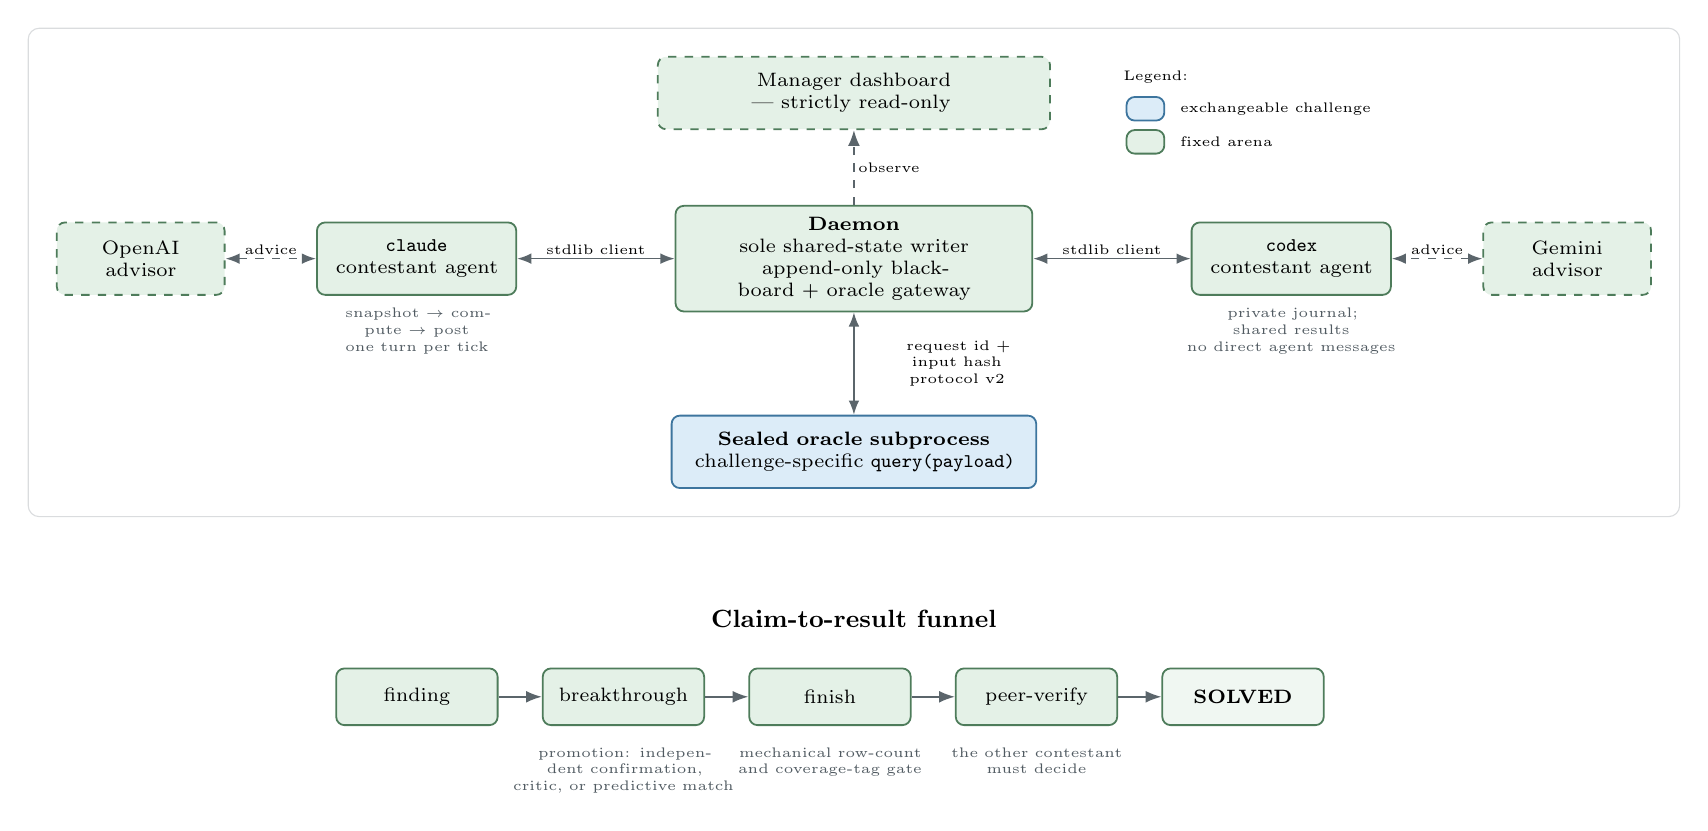
\begin{tikzpicture}[
  font=\scriptsize,
  fixed/.style={rounded corners=3pt,draw=HarnessLine,fill=HarnessGreen,
    line width=0.65pt,align=center,minimum height=0.92cm,inner sep=4pt},
  inst/.style={rounded corners=3pt,draw=InstanceLine,fill=InstanceBlue,
    line width=0.65pt,align=center,minimum height=0.92cm,inner sep=4pt},
  aux/.style={fixed,dashed},
  gate/.style={fixed,minimum width=2.05cm,minimum height=0.72cm},
  flow/.style={-{Latex[length=2mm]},draw=Ink!75,line width=0.6pt},
  twoway/.style={{Latex[length=1.8mm]}-{Latex[length=1.8mm]},
    draw=Ink!75,line width=0.6pt},
  dashedflow/.style={flow,dashed},
  label/.style={font=\tiny,fill=white,inner sep=1.3pt,align=center},
  note/.style={font=\tiny,align=center,text=Ink!80}
]
  \node[fixed,text width=4.25cm,minimum height=1.30cm] (daemon)
    {\textbf{Daemon}\\sole shared-state writer\\append-only blackboard +
    oracle gateway};
  \node[fixed,text width=2.25cm,left=2.0cm of daemon] (claude)
    {\code{claude}\\contestant agent};
  \node[fixed,text width=2.25cm,right=2.0cm of daemon] (codex)
    {\code{codex}\\contestant agent};
  \node[aux,text width=1.85cm,left=1.15cm of claude] (openai)
    {OpenAI\\advisor};
  \node[aux,text width=1.85cm,right=1.15cm of codex] (gemini)
    {Gemini\\advisor};
  \node[aux,text width=4.7cm,above=0.95cm of daemon] (manager)
    {Manager dashboard --- strictly read-only};
  \node[inst,text width=4.35cm,below=1.30cm of daemon] (oracle)
    {\textbf{Sealed oracle subprocess}\\challenge-specific
    \code{query(payload)}};

  \draw[twoway] (claude) -- node[label,above]{stdlib client} (daemon);
  \draw[twoway] (codex) -- node[label,above]{stdlib client} (daemon);
  \draw[twoway,dashed] (openai) -- node[label,above]{advice} (claude);
  \draw[twoway,dashed] (gemini) -- node[label,above]{advice} (codex);
  \draw[dashedflow] (daemon) -- node[label,right]{observe} (manager);
  \draw[twoway] (daemon) -- node[label,right,text width=2.5cm]
    {request id + input hash\\protocol v2} (oracle);

  \node[note,below=1pt of claude,text width=2.9cm]
    {snapshot $\to$ compute $\to$ post\\one turn per tick};
  \node[note,below=1pt of codex,text width=2.9cm]
    {private journal; shared results\\no direct agent messages};

  \node[font=\small\bfseries,below=1.42cm of oracle] (funnel)
    {Claim-to-result funnel};
  \node[gate,below=0.38cm of funnel,xshift=-5.55cm] (finding) {finding};
  \node[gate,right=0.55cm of finding] (breakthrough) {breakthrough};
  \node[gate,right=0.55cm of breakthrough] (finish) {finish};
  \node[gate,right=0.55cm of finish] (verify) {peer-verify};
  \node[gate,right=0.55cm of verify,fill=HarnessGreen!55] (solved)
    {\textbf{SOLVED}};
  \draw[flow] (finding)--(breakthrough);
  \draw[flow] (breakthrough)--(finish);
  \draw[flow] (finish)--(verify);
  \draw[flow] (verify)--(solved);

  \node[note,below=0.15cm of breakthrough,text width=3.6cm]
    {promotion: independent confirmation,\\critic, or predictive match};
  \node[note,below=0.15cm of finish,text width=2.8cm]
    {mechanical row-count\\and coverage-tag gate};
  \node[note,below=0.15cm of verify,text width=2.4cm]
    {the other contestant\\must decide};

  \node[anchor=west,font=\tiny] at ($(manager.east)+(0.8,0.2)$) {Legend:};
  \node[inst,minimum width=0.48cm,minimum height=0.30cm,inner sep=0pt]
    at ($(manager.east)+(1.2,-0.2)$) {};
  \node[anchor=west,font=\tiny] at ($(manager.east)+(1.52,-0.2)$)
    {exchangeable challenge};
  \node[fixed,minimum width=0.48cm,minimum height=0.30cm,inner sep=0pt]
    at ($(manager.east)+(1.2,-0.62)$) {};
  \node[anchor=west,font=\tiny] at ($(manager.east)+(1.52,-0.62)$)
    {fixed arena};

  \begin{scope}[on background layer]
    \node[draw=Ink!17,rounded corners=4pt,
      fit=(openai)(gemini)(manager)(oracle),inner sep=10pt] {};
  \end{scope}
\end{tikzpicture}}
\caption{Layer A topology and claim funnel.  The fixed daemon is sovereign
over writes and oracle access; contestants coordinate through append-only
state, not conversation.  The blue oracle belongs to the exchangeable
challenge package.  A claim must cross promotion, a mechanically parsed
finish gate when configured, and verification by the other contestant before
the daemon writes \code{SOLVED}.}
\label{fig:arena}
\end{figure}

\section{Layer A: the arena}

\subsection{Sovereignty and process boundaries}

The daemon is the only process allowed to mutate shared state.  Every
contestant action is an HTTP request from the stdlib-only client; handlers
serialize writes through the state manager.  The daemon never imports the
challenge oracle.  It starts a worker subprocess, exchanges one JSON object
per line, and exposes only the returned answer.  This boundary prevents an
ordinary import from turning the answer key into contestant context.

The seal is a process and protocol boundary, not an operating-system sandbox.
An agent with unrestricted file access must still be instructed not to inspect
the oracle source.  The important architectural property is that normal
contestant operation needs no such access and all accepted oracle evidence
passes through one audited path.

\subsection{Tick discipline and stigmergy}

Each contestant executes the same stateless tick: pull a journal-first
snapshot, compute, optionally query, append a finding or promotion candidate,
update private direction and journal, append a turn record, and yield.
Contestants do not direct one another.  Their discoveries become environmental
signals on the shared blackboard.  This stigmergic structure preserves
participant-level independence: routes are developed privately, while
results become visible enough to support corroboration and critique.

The state split is deliberate.  A contestant's journal and current direction
preserve continuity across short contexts.  Shared findings,
breakthroughs, finish records, and oracle logs are append-only.  A round
counter advances only when a turn record is posted, making missing ticks
visible.

\subsection{Predict before query}

An oracle request may carry both a proposed output and the hypothesis that a
match would support.  The prediction is written before a new execution.
After a correlated response, exact JSON equality determines whether it
matched.  When the challenge enables predictive promotion, a successful
prediction can promote the hypothesis without relying on retrospective
storytelling.  Plain queries remain available for calibration, but prediction
turns a lookup into a falsifiable test.

\subsection{Request correlation, cache versions, and trust epochs}

Every worker response must round-trip the protocol version, challenge name,
request id, and a hash of the canonical JSON input.  The runner rejects a
mismatch, restarts the worker, and retries once.  An executed log record also
stores a cache version and an \code{oracle\_protocol\_verified} flag.  Cache
lookup accepts only a current-version record whose metadata matches the
requested input.  Older records remain visible but are demoted to a legacy
trust epoch and cannot supply ground truth.

\paragraph{Anonymized incident.}
In an earlier run, a stale response was attributed to the next request and
poisoned the ground-truth cache.  A later recomputation disagreed.  Because
the oracle log was append-only, the operator reconstructed the fault
line-by-line, identified the first misattribution, and separated downstream
claims that had consumed it.  The repair added request-id and input-hash
correlation, versioned the cache, and demoted every pre-fix record.  No record
was erased.  The incident is why the oracle channel is treated as evidence
that must itself be verified.

\subsection{The claim funnel}

Figure~\ref{fig:arena} shows five states.  Findings are open observations.
Breakthrough candidates have three possible promotion paths:

\begin{enumerate}[leftmargin=*,itemsep=0.2em]
\item \textbf{Independent confirmation.}  A different contestant has already
posted a substantially overlapping claim.
\item \textbf{Adversarial critic.}  A separate verifier judges the candidate
against the oracle evidence it cites.  This path fails closed if its external
command is unavailable.
\item \textbf{Predictive match.}  A preregistered oracle prediction succeeds
and promotes the attached hypothesis.
\end{enumerate}

A finish is a complete effective algorithm plus a correctness argument.  If
the challenge declares \code{finish\_gate}, each evidence row must parse in
the pinned format and matching rows must meet both the minimum count and every
required coverage tag.  A malformed row rejects the submission before it can
enter peer verification.  When no finish gate is declared, the original
direct-to-peer behavior is retained.  Historically, 18 of 32 finish
proposals were rejected with concrete counterexamples; acceptance therefore
cannot be inferred from fluency or persistence.

Only another contestant may verify a finish.  Agreement causes the daemon to
write \code{SOLVED}; rejection requires a concrete reason.  Retractions and
superseding proposals append new records.  A stale victory marker is evidence
about history and is not silently removed.

\clearpage

\subsection{Supporting roles}

The advisor is cross-vendor and reserved for hard derivations or direction
checks.  It never substitutes for oracle evidence.  Its persistent spend
ledger uses a file lock and a conservative pre-call reservation; any call
that could exceed the hard dollar cap is refused before network activity.
The OpenAI and Gemini SDKs are optional and imported only in the selected
advisor path, so the daemon has no advisor dependency.

The optional historian periodically summarizes active threads, dead ends,
and open questions.  Its prompt forbids instructions: it is non-directive by
construction.  The manager and status views read files and health data only;
they expose no mutation endpoint.  The demo disables both historian and critic
commands, so its retest invokes no external model or agent CLI.

\subsection{Append-only reproducibility}

Findings, breakthroughs, finishes, verifications, turns, and oracle events
are JSONL records with human-readable mirrors.  JSONL append flushes and
synchronizes each line.  Corrections are new records, and \code{SOLVED} is
published atomically.  State therefore reconstructs the research sequence,
including failed predictions, rejected finishes, and trust-epoch changes.

\begin{table}[htbp]
\centering
\small
\caption{Arena state surfaces and mutation rules.}
\label{tab:arena-state}
\begin{tabularx}{\textwidth}{@{}
  >{\raggedright\arraybackslash}p{0.28\textwidth}
  >{\raggedright\arraybackslash}p{0.24\textwidth}Y@{}}
\toprule
Surface & Writer & Reproducibility rule \\
\midrule
\code{shared/findings.*} &
daemon finding handler &
Append one open observation; corrections add a later finding. \\
\code{shared/breakthroughs.*} &
daemon promotion path &
Append only after the promotion reason has been fixed. \\
\code{shared/finish.*} &
daemon finish and verify handlers &
Append proposal and verdict as separate records. \\
\code{shared/oracle\_log.*} &
daemon oracle handler &
Append prediction and execution separately; retain protocol metadata. \\
\code{contestants/<id>/} &
daemon continuity handlers &
Journal and turns append; current direction is the sole replaceable view. \\
\code{round\_counter.txt}, \code{SOLVED} &
daemon only &
Increment the round under lock; publish the solved record atomically. \\
\bottomrule
\end{tabularx}
\end{table}

\clearpage

\section{Layer B: the evidence kit}

The arena gates acceptance; the evidence kit gates evidence quality.  It is
used while preparing a finish and again after acceptance to consolidate the
algorithm into checked claims.  The fixed package \code{gauntlet/} supplies
manifests, policies, gates, provenance, a sequential runner, independence
lint, reports, and table generation.  An exchangeable instance supplies the
mathematics.

\begin{figure}[htbp]
\centering
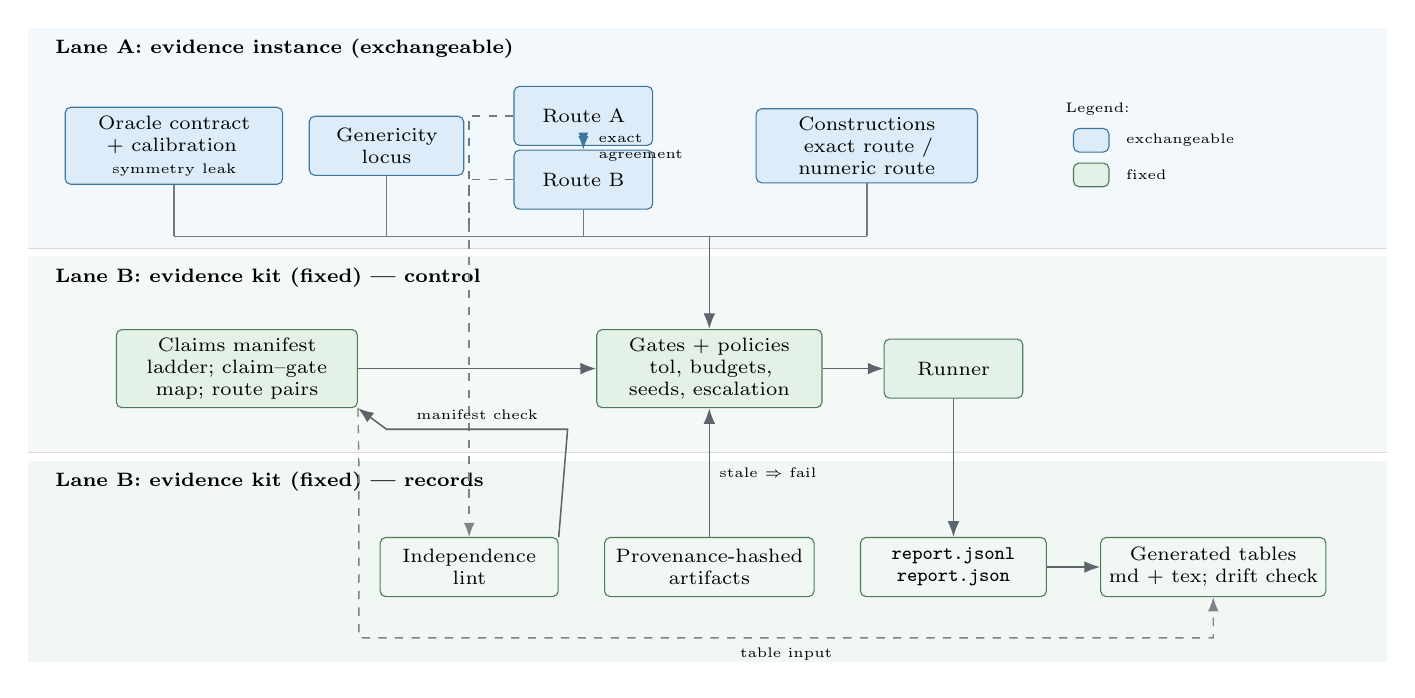
\begin{tikzpicture}[
  x=1cm,y=1cm,
  font=\scriptsize,
  flow/.style={-{Latex[length=2mm]},draw=Ink!75,line width=0.55pt},
  wire/.style={draw=Ink!65,line width=0.5pt},
  read/.style={-{Latex[length=1.8mm]},draw=Ink!60,dashed,line width=0.5pt},
  inst/.style={rounded corners=2pt,draw=InstanceLine,fill=InstanceBlue,
    minimum height=0.75cm,align=center,inner sep=3pt},
  fixed/.style={rounded corners=2pt,draw=HarnessLine,fill=HarnessGreen,
    minimum height=0.75cm,align=center,inner sep=3pt},
  data/.style={rounded corners=2pt,draw=HarnessLine,fill=EvidenceGreen,
    minimum height=0.75cm,align=center,inner sep=3pt}
]
  \fill[InstanceBlue!38] (0,5.25) rectangle (17.25,8.05);
  \fill[HarnessGreen!42] (0,2.65) rectangle (17.25,5.15);
  \fill[EvidenceGreen] (0,0) rectangle (17.25,2.55);
  \draw[Ink!18] (0,5.25)--(17.25,5.25);
  \draw[Ink!18] (0,2.65)--(17.25,2.65);

  \node[anchor=west,font=\bfseries\scriptsize] at (0.22,7.78)
    {Lane A: evidence instance (exchangeable)};
  \node[anchor=west,font=\bfseries\scriptsize] at (0.22,4.88)
    {Lane B: evidence kit (fixed) --- control};
  \node[anchor=west,font=\bfseries\scriptsize] at (0.22,2.28)
    {Lane B: evidence kit (fixed) --- records};

  \node[inst,text width=2.55cm] (oracle2) at (1.85,6.55)
    {Oracle contract + calibration\\{\tiny symmetry leak}};
  \node[inst,text width=1.75cm] (generic) at (4.55,6.55)
    {Genericity\\locus};
  \node[inst,text width=1.55cm] (routea) at (7.05,6.93) {Route A};
  \node[inst,text width=1.55cm] (routeb) at (7.05,6.12) {Route B};
  \draw[{Latex[length=1.7mm]}-{Latex[length=1.7mm]},double,
    double distance=0.7pt,draw=InstanceLine]
    (routea.south) -- node[right=2pt,align=left,font=\tiny]
    {exact\\agreement} (routeb.north);
  \node[inst,text width=2.6cm] (builds) at (10.65,6.55)
    {Constructions\\exact route / numeric route};

  \node[fixed,text width=2.85cm] (manifest) at (2.65,3.72)
    {Claims manifest\\ladder; claim--gate map; route pairs};
  \node[fixed,text width=2.65cm] (gates) at (8.65,3.72)
    {Gates + policies\\tol, budgets, seeds, escalation};
  \node[fixed,text width=1.55cm] (runner) at (11.75,3.72) {Runner};

  \node[data,text width=2.05cm] (lint) at (5.60,1.20)
    {Independence\\lint};
  \node[data,text width=2.45cm] (artifacts) at (8.65,1.20)
    {Provenance-hashed\\artifacts};
  \node[data,text width=2.15cm] (reports) at (11.75,1.20)
    {\code{report.jsonl}\\\code{report.json}};
  \node[data,text width=2.65cm] (tables) at (15.05,1.20)
    {Generated tables\\md + tex; drift check};

  \draw[flow] (manifest.east) -- (gates.west);
  \draw[flow] (gates.east) -- (runner.west);
  \draw[flow] (runner.south) -- (reports.north);
  \draw[flow] (reports.east) -- (tables.west);
  \draw[flow] (artifacts.north) -- node[right,font=\tiny]
    {stale $\Rightarrow$ fail} (gates.south);
  \coordinate (routejoin) at (5.60,5.56);
  \draw[wire,dashed] (routea.west) -- (5.60,6.93) -- (routejoin);
  \draw[wire,dashed] (routeb.west) -- (5.60,6.12) -- (routejoin);
  \draw[read] (routejoin) -- (lint.north);
  \draw[flow] (lint.north east) -- (6.85,2.95) --
    node[above,font=\tiny] {manifest check} (4.55,2.95) --
    (manifest.south east);

  \coordinate (inputbus) at (8.65,5.40);
  \draw[wire] (1.85,5.40) -- (10.65,5.40);
  \draw[wire] (oracle2.south) -- (1.85,5.40);
  \draw[wire] (generic.south) -- (4.55,5.40);
  \draw[wire] (routeb.south) -- (7.05,5.40);
  \draw[wire] (builds.south) -- (10.65,5.40);
  \draw[flow] (inputbus) -- (gates.north);
  \draw[read] (manifest.south east) -- (4.20,2.45) -- (4.20,0.30) --
    node[below,font=\tiny] {table input} (15.05,0.30) -- (tables.south);

  \node[anchor=west,font=\tiny] at (13.05,7.02) {Legend:};
  \node[inst,minimum width=0.45cm,minimum height=0.3cm,inner sep=0pt]
    at (13.50,6.62) {};
  \node[anchor=west,font=\tiny] at (13.82,6.62) {exchangeable};
  \node[fixed,minimum width=0.45cm,minimum height=0.3cm,inner sep=0pt]
    at (13.50,6.18) {};
  \node[anchor=west,font=\tiny] at (13.82,6.18) {fixed};
\end{tikzpicture}
\caption{Layer B claim-coupled pipeline.  Exchangeable reconstruction and
construction modules feed fixed policies and gates.  Structured records,
provenance checks, import lint, and generated tables close the loop between
claims, executable evidence, and the writeup.}
\label{fig:evidence}
\end{figure}

\subsection{Redundant ground truth and the claim ladder}

An evidence instance reconstructs the identified object by at least two
substantively independent routes.  Exact objects use integer or rational
arithmetic; structural facts become assertions rather than comments.  The
manifest declares route pairs and forbidden shared imports, while an AST lint
checks direct dependencies.  The lint is a mechanical backstop, not a proof
of conceptual independence.

Each claim occupies one rung:
\code{conjectured}, \code{numeric}, \code{exact},
\code{proved\_small}, or \code{proved}.  Promotion needs evidence appropriate
to the new rung.  A weakened or removed gate forces demotion to the highest
still-supported rung.  Proof rungs require a proof link; cheap executable
checks remain valuable as regression evidence even after proof.

\subsection{Gates, policy, and explicit coverage}

A gate covers one claim or one tight claim group.  Its policy owns tolerances,
sample counts, time budgets, quick-mode scaling, size ladders, and precision
stages.  Random streams derive from a root seed and stable gate identifier:

\begin{equation}
s_g=\operatorname{int}_{\mathrm{big}}
\left(\operatorname{SHA256}(\operatorname{text}(s)\mathbin{:}g)[0{:}8]\right).
\label{eq:gate-seed}
\end{equation}

Equation~\ref{eq:gate-seed} makes a gate's stream independent of registry
ordering.  Root and derived seeds are recorded.  Every coverage reduction is
an explicit \code{SKIP} with a reason.  A false check produces
\code{FAIL}; an unhandled exception becomes a failing structured check and
does not prevent later gates from running.

\subsection{JSONL schema}

The runner writes one JSON object per line and a matching aggregate JSON
object.  Table~\ref{tab:schema} is the stable record surface.

\begin{table}[htbp]
\centering
\small
\caption{Record fields in \code{report.jsonl}.}
\label{tab:schema}
\begin{tabularx}{\textwidth}{@{}p{0.13\textwidth}Y Y@{}}
\toprule
Record & Fields & Purpose \\
\midrule
\code{meta} &
\code{type}, \code{instance}, \code{root\_seed}, \code{quick},
\code{started\_utc} &
Run identity and root settings. \\
\code{check} &
\code{type}, \code{gate\_id}, \code{name}, \code{config},
\code{verdict}, \code{criterion}, \code{measured}, \code{runtime\_s},
\code{extra} &
One atomic probe, including measured data and error detail. \\
\code{gate} &
\code{type}, \code{gate\_id}, \code{title}, \code{claim\_ids},
\code{verdict}, pass/fail/skip counts, \code{runtime\_s}, \code{seed},
\code{policy\_snapshot} &
Gate roll-up and the exact policy used. \\
\code{summary} &
\code{type}, \code{ok}, \code{totals} &
Final run verdict and aggregate counts. \\
\bottomrule
\end{tabularx}
\end{table}

\subsection{Artifacts, generated tables, and drift}

An expensive artifact carries its payload, creation data, producer-code
hashes, and caller metadata.  Loading recomputes every declared hash.  A
missing producer or unequal digest marks the artifact stale, and a consuming
gate fails until an explicit rebuild occurs.

The table generator joins the manifest to the latest report and emits
Markdown and LaTeX.  It never upgrades a claim; it makes claim-to-gate
linkage visible.  The drift conditions are fixed in
Table~\ref{tab:drift}.

\begin{table}[htbp]
\centering
\small
\caption{Writeup drift conditions and their meaning.}
\label{tab:drift}
\begin{tabularx}{\textwidth}{@{}p{0.43\textwidth}Y@{}}
\toprule
Condition & Why it is rejected \\
\midrule
A claim names a gate missing from the report. &
The documented claim has no executed evidence in this run. \\
An exact or proof-rung claim has no passing linked check. &
The status outruns its current evidence. \\
A report gate is not claimed by the manifest. &
Executed work is detached from the published claim surface. \\
Any report check has verdict \code{FAIL}. &
The generated document must expose, not conceal, the failure. \\
\bottomrule
\end{tabularx}
\end{table}

\clearpage

\section{Exchangeable demonstrations and retests}

\subsection{\exchangeable: Layer A demo challenge}

\code{challenges/ising\_lift/} is a worked arena package.  Inputs are weighted
graphs with integer edge couplings and integer vertex fields.  The sealed
oracle exhaustively enumerates binary sign assignments for sizes up to
sixteen.  It reports \code{wall} if any assignment is degenerate; otherwise
it returns the difference between positive and negative classical counts.
The contestant statement deliberately describes only the graph contract,
five calibration values, and a change-of-variables leak.  It withholds the
Ising interpretation, which is part of the discovery task.

The finish must identify a Laurent-polynomial lift, give an effective
coefficient algorithm, justify the extraction of the classical coefficient,
and include at least twelve matching evidence rows.  Required tags force
coverage at sizes two through five, with and without fields, the deliberate
leak pair, a frustrated case, a wall check, and a disconnected graph.

\subsection{\exchangeable: Layer A scripted retest}

\code{arena/smoke\_arena.py} is orchestration, not a substitute contestant.
It starts the daemon with its own interpreter and a temporary
\code{ORACLE\_STATE\_ROOT}, then invokes the real stdlib client as
\code{claude} and \code{codex}.  It uses localhost only.  The retest asserts
the stages in Table~\ref{tab:smoke}.

\begin{table}[htbp]
\centering
\small
\caption{Deterministic arena retest coverage.}
\label{tab:smoke}
\begin{tabularx}{\textwidth}{@{}p{0.08\textwidth}Y@{}}
\toprule
Step & Assertion surface \\
\midrule
1 & Health, served problem text, enabled oracle, and no hidden interpretation
words in the contestant statement. \\
2 & Seven pinned oracle cases, including integer and wall outputs, with
request ids and input hashes. \\
3 & A matching prediction promotes a breakthrough with reason
\code{predictive\_match}. \\
4 & A second contestant's overlapping finding promotes a claim through
independent confirmation. \\
5 & A finish without evidence is rejected before any verification record is
created. \\
6 & Twelve live-query rows cover every configured tag and enter peer
verification. \\
7 & The other contestant agrees; daemon health and the marker both report
\code{SOLVED}. \\
8 & Shared JSONL and Markdown mirrors, private continuity files, turn records,
round count, and monotone line counts satisfy the state layout. \\
9 & The daemon terminates and the temporary state root is removed. \\
\bottomrule
\end{tabularx}
\end{table}

The shipped run completes all nine stages with 219 assertions in well under
two minutes and makes no external API or agent-CLI call.  Because it queries
the challenge oracle through the same daemon and client used by real agents,
it retests both the mathematical fixture and the operational funnel.

\subsection{\exchangeable: Layer B worked instance}

\code{example\_ising/} is the consolidation-side demonstration.  It provides
two reconstruction routes, exact and numeric construction checks, symmetry
tests, a provenance-coupled finite census, and generated tables.  The full
stdlib run reports seven gates and 300 passing checks, with zero failures,
zero skips, and a clean drift result.  The specific constructions are
replaceable; the manifest, gate context, runner, provenance rules, and report
format remain fixed.

\section{Authoring and swap contract}

Layer A and Layer B are independently exchangeable.

\paragraph{Layer A.}
Copy \code{challenges/\_template/}, rename the directory, and make
\code{challenge.name} agree.  Write the contestant task and calibration leak
in \code{problem.md}; define schemas, promotion, and optional evidence
coverage in \code{config.yaml}; implement sealed \code{query(payload)} in
\code{oracle.py}.  The template includes a commented finish-gate example.

\paragraph{Layer B.}
Copy \code{instance\_template/}, implement two oracle routes, genericity and
calibration modules, construction modules, gates, and
\code{manifest\_def.py}.  Select the package with
\code{python3 run\_demo.py --instance NAME}.  Any costly product consumed by
a gate must use provenance-coupled artifact I/O, and the generated
verification tables must be included without hand editing.

\begin{table}[htbp]
\centering
\small
\caption{Swap boundary for the two layers.}
\label{tab:swap}
\begin{tabularx}{\textwidth}{@{}p{0.18\textwidth}Y Y@{}}
\toprule
Layer & Exchangeable package & Fixed machinery \\
\midrule
A: discovery &
\code{problem.md}, \code{config.yaml}, \code{oracle.py} &
daemon, client, correlated oracle protocol, state manager, promotion,
historian, advisors, dashboard, status, and ops. \\
B: consolidation &
oracle routes, calibration, genericity, constructions, gates, manifest &
gate context, policy, runner, provenance, independence lint, JSONL reports,
table generator, and drift check. \\
\bottomrule
\end{tabularx}
\end{table}

\subsection{Layer A author checks}

Before a challenge is admitted to a real contest, its author checks the
boundary rather than only the answer values:

\begin{enumerate}[leftmargin=*,itemsep=0.2em]
\item The directory slug and \code{challenge.name} agree, both schemas
validate, and every configured contestant id is accepted by the client.
\item Direct oracle calls cover valid, malformed, and wall cases.  The worker
returns the same request metadata that the runner sent, and a deliberately
altered request id or input hash is rejected.
\item Calibration contains a real symmetry-linked pair, while
\code{problem.md} does not disclose the construction that contestants are
meant to identify.
\item The finish gate, when used, has attainable but nontrivial tags.  One
valid matrix passes; missing rows, missing tags, malformed JSON, and a
nonmatching row produce clear failures before peer review.
\item Historian and critic settings match the operating environment.
Demonstrations that promise offline behavior disable both external command
paths.
\end{enumerate}

\subsection{Layer B author checks}

The consolidation package is accepted only when both routes reproduce every
calibration row and seeded sweep, route lint reports no forbidden direct
import, each claim names an existing gate, and every proof rung names a proof
reference.  Quick mode may reduce counts but must emit explicit coverage
records.  The full run must recreate or validate every consumed artifact,
write parseable JSONL through the final summary, generate both table formats,
and return a clean drift result.

The swap test is therefore behavioral.  Renaming a package is insufficient:
the author demonstrates that fixed code can load it, that all failure paths
remain fail-closed, and that the resulting records can explain both a success
and an intentional failure without hand repair.

\section{Operating procedure P0--P6}

\begin{description}[style=nextline,leftmargin=1.3cm,labelwidth=1.1cm,itemsep=0.35em]
\item[P0 --- Author.]
Copy the Layer A template.  Write the task, symmetry-linked calibration,
finish criteria, schemas, promotion policy, evidence coverage, and sealed
oracle.  Version the package; keep runtime state and scratch data untracked.

\item[P1 --- Boot.]
Start the daemon and verify health.  Contestants retrieve the problem through
the client and confirm the oracle mode.

\item[P2 --- Contest.]
Run independent ticks.  Use cross-vendor advisors only for difficult
derivations, predict before informative queries, post results to the
blackboard, and let configured promotion paths operate.

\item[P3 --- Finish.]
Assemble the effective algorithm, correctness argument, and evidence matrix.
The daemon applies the mechanical gate; the other contestant verifies or
rejects with a concrete gap.

\item[P4 --- Solve.]
Only the daemon, and only after peer agreement, writes \code{SOLVED}.

\item[P5 --- Consolidate.]
Move the accepted algorithm into an evidence-kit instance.  Build two routes,
claim-sized gates, ladder statuses, provenance-coupled artifacts, and
generated tables.  Promote only what the evidence supports.

\item[P6 --- Ship.]
Publish reproduction commands, generated tables, the reconstructible
discovery history, and the open frontier.
\end{description}

\clearpage

\section{Failure modes and defenses}

\begin{table}[htbp]
\centering
\footnotesize
\caption{Failure modes addressed across both layers.}
\label{tab:failures}
\begin{tabularx}{\textwidth}{@{}p{0.34\textwidth}Y@{}}
\toprule
Failure mode & Defense \\
\midrule
Premature victory or self-certification &
Peer verification by the other contestant; daemon-set \code{SOLVED}; stale
markers retained. \\
Plausible but wrong claims &
Three promotion paths, prediction before query, and an adversarial critic. \\
Groupthink or shared blind spots &
Cross-vendor contestants and advisors, private construction, and stigmergic
rather than conversational coordination. \\
Gamed or thin finish evidence &
Mechanical row count and coverage tags before verification. \\
Oracle-channel corruption &
Request id and input hash on every response, versioned cache, recomputation,
and trust epochs. \\
Shared-state corruption or lost history &
Single-writer daemon, append-only logs, and superseding corrections. \\
Runaway advisor spend &
Fail-closed hard-cap ledger with pre-call reservation. \\
Context drift over long runs &
Journal-first snapshots and non-directive historian digests. \\
Convention or sign errors in consolidation &
Two independent routes, symmetry invariants, and the calibration leak. \\
Writeup drift from the suite &
Generated verification tables and the drift check. \\
Silent coverage loss &
Explicit \code{SKIP} records with reasons. \\
Stale cached artifacts &
Producer hashes checked by every consuming gate. \\
Irreproducible randomness &
Root seed, stable per-gate derivation, and recorded seeds. \\
\bottomrule
\end{tabularx}
\end{table}

\section{Reproducibility surface}

A complete run has two audit trails.  The arena state records how the result
was discovered and accepted: private continuity, shared claims, oracle
traffic, finish decisions, and rounds.  The evidence report records how the
accepted construction was checked: meta settings, atomic checks, gate
roll-ups, summary totals, artifacts, and the generated claim table.  The two
trails answer different questions and should not be collapsed.  Peer
agreement is not a proof, and a green consolidation suite does not recreate
the independent discovery history.

The shipped reproduction commands are intentionally short:

\begin{quote}
\small\ttfamily
python3 -m venv .venv\\
.venv/bin/pip install -r arena/requirements.txt\\
.venv/bin/python arena/smoke\_arena.py\\
python3 run\_demo.py\\
make -C report
\end{quote}

The arena retest creates and removes its own state root.  The evidence run is
standard-library-only.  The report build is separate so operational state,
verification records, and typeset prose cannot silently substitute for one
another.

\section{Limitations}

Version 0.2 does not bundle autonomous contestant runners.  The operator
starts and supervises each agent loop, while the daemon remains passive.
Layer B executes gates sequentially; isolated contexts and derived seeds make
parallel scheduling possible, but it is not implemented.  Compute offload is
also operator-managed: policy budgets record intent, yet no runner currently
routes a heavy job to another machine.

Proof-rung claims cite human-checked proofs through \code{proof\_ref}; there
is no formal-proof integration.  There is no CI configuration.  The existing
exit codes, JSONL records, deterministic seeds, smoke script, and build
commands are suitable inputs to CI, but shipping such a wrapper would add an
operational policy not required by the method.

These limits narrow automation, not the epistemic contract.  The daemon still
owns acceptance, the peer remains independent, the oracle channel remains
correlated, evidence cuts remain explicit, stale products fail closed, and
the published claim status cannot outrun its checked support.

Several boundaries remain deliberately human-facing.  The finish gate checks
syntax, row count, matching declarations, and tag coverage; it does not prove
that a proposed value was derived honestly or that the algorithm generalizes.
The peer must compare the cited rows with the shared oracle history and must
inspect the correctness argument.  Likewise, a passing numeric gate supports
only the policy and domain it records.  It cannot be described as exact
evidence without a separate exact route.

The sealed worker prevents accidental imports through the normal arena path,
but it is not a hostile-code container.  A contestant granted unrestricted
filesystem access could violate the protocol by reading challenge source.
Real deployments must pair the software boundary with agent instructions or
an operating-system sandbox appropriate to their threat model.  The
challenge author also remains trusted to implement the stated oracle
contract; schema validation cannot establish that the answer key itself is
mathematically correct.

Finally, direct-import lint detects obvious route coupling but not shared
ideas, copied logic, or transitive dependencies.  Cross-vendor roles reduce
correlated error without proving independence.  Review therefore remains
necessary at three points: challenge authoring, peer acceptance, and any
promotion to a proof rung.  The method records those judgments so they can be
audited; it does not pretend to automate them away.

\section{Conclusion}

The two layers separate discovery risk from evidence risk without separating
their records.  The arena makes independent agents earn a result through
prediction, promotion, a mechanical evidence threshold, and adversarial peer
review.  The evidence kit then turns that result into reproducible,
claim-sized checks with an honest proof frontier.  Challenge packages and
evidence instances can change; daemon sovereignty, append-only history,
request correlation, independent routes, provenance, and generated tables
remain the fixed method.

\end{document}
